\section{Movimiento en una dimensión}
  \subsection{Posición, velocidad y repidez}
    \begin{itemize}
      \item La \textbf{posición} x de una partícula es la ubicación de la partícula respecto a un punto de referencia
      elegido que se considera el origen de un sistema coordenado. El movimiento de una partícula se conoce por completo
      si la posición de la partícula en el espacio se conoce en todo momento.

      \item El \textbf{desplazamiento} $\Delta x$ de una partícula se define como su cambio en posición en algún
      intervalo de tiempo. Conforme la partícula se mueve desde una posición inicial $x_{i}$ a una posición final
      $x_{f}$, su desplazamiento está dado por:
      \begin{equation*}
        \Delta x \equiv x_{f} - x_{i}
      \end{equation*}

      \item \textbf{Distancia} es la longitud de una trayectoria seguida por una partícula. La distancia siempre se
      representa como un número positivo, mientras que el desplazamiento puede ser positivo o negativo.
4
      \item La \textbf{velocidad promedio} $v_{x,prom}$ de una partícula se define como el desplazamiento x de la
      partícula dividido entre el intervalo de tiempo $t$ durante el que ocurre dicho desplazamiento:
      \begin{equation*}
        v_{x,prom} \equiv \frac{\Delta x}{\Delta t}
      \end{equation*}

      \item La \textbf{rapidez promedio} $v_{prom}$ de una partícula, una cantidad escalar, se define como la distancia
      total recorrida dividida entre el intervalo de tiempo total requerido para recorrer dicha distancia:
      \begin{equation*}
        v_{prom} \equiv \frac{d}{\Delta t}
      \end{equation*}
    \end{itemize}

  \subsection{Velocidad y rapidez instantáneas}
    \begin{itemize}
      \item La \textbf{velocidad instantánea} $v_{x}$ es igual al valor límite de la razón $\Delta x / \Delta t$
      conforme $\Delta t$ tiende a cero, es decir, a la derivada de x respecto de $t$:
      \begin{equation*}
        v_{x} \equiv \lim_{\Delta t \rightarrow 0} \ \frac{\Delta x}{\Delta t} = \frac{dx}{dt}
      \end{equation*}

      \item La \textbf{rapidez instantánea} de una partícula se define como la magnitud de su velocidad instantánea.
    \end{itemize}

  \subsection{Aceleración}
    \begin{itemize}
      \item La \textbf{aceleración promedio} $a_{x,prom}$ de la partícula se define como el cambio en velocidad $\Delta
      v_{x}$ dividido entre el intervalo de tiempo $t$ durante el que ocurre el cambio:
      \begin{equation*}
        a_{x,prom} \equiv \frac{\Delta v_{x}}{\Delta t} = \frac{v_{xf} - v_{xi}}{t_{f} - t_{i}}
      \end{equation*}

      \item La \textbf{aceleración instantánea} como el límite de la aceleración promedio conforme $\Delta t$ tiende a
      cero.
      \begin{equation*}
        a_{x} \equiv \lim_{\Delta t \rightarrow 0} \ \frac{\Delta v_{x}}{\Delta t} = \frac{dv_{x}}{dt} =
        \frac{d^{2}x}{dt^{2}}
      \end{equation*}
    \end{itemize}

  \subsection{Análisis de modelos}
    \begin{figure}[H]
      \centering
      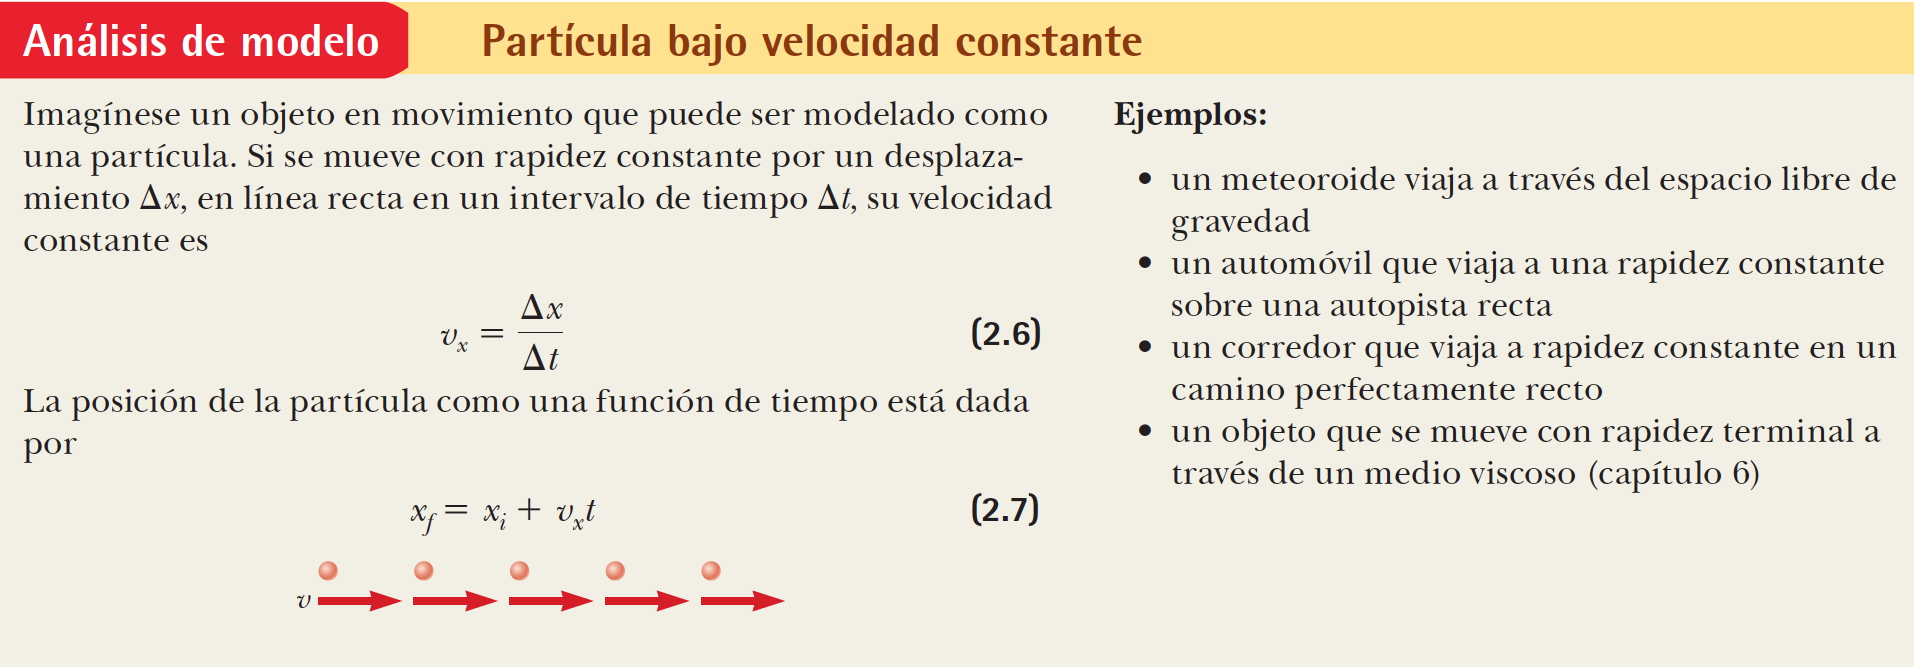
\includegraphics[scale=0.5]{1/graphics_2/figure_0a}
    \end{figure}
    \begin{figure}[H]
      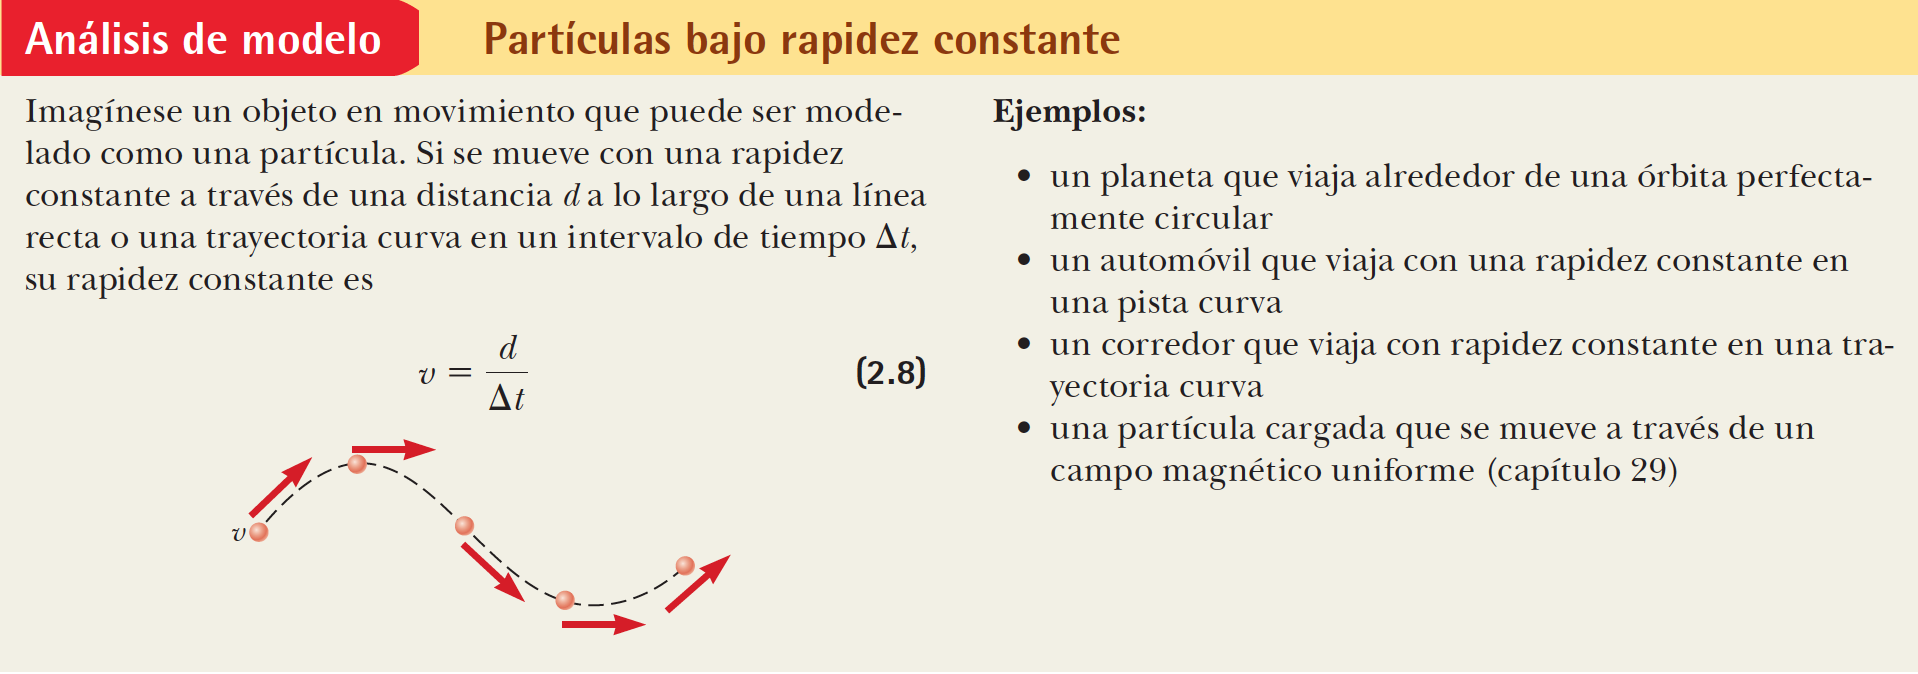
\includegraphics[scale=0.5]{1/graphics_2/figure_0b}
      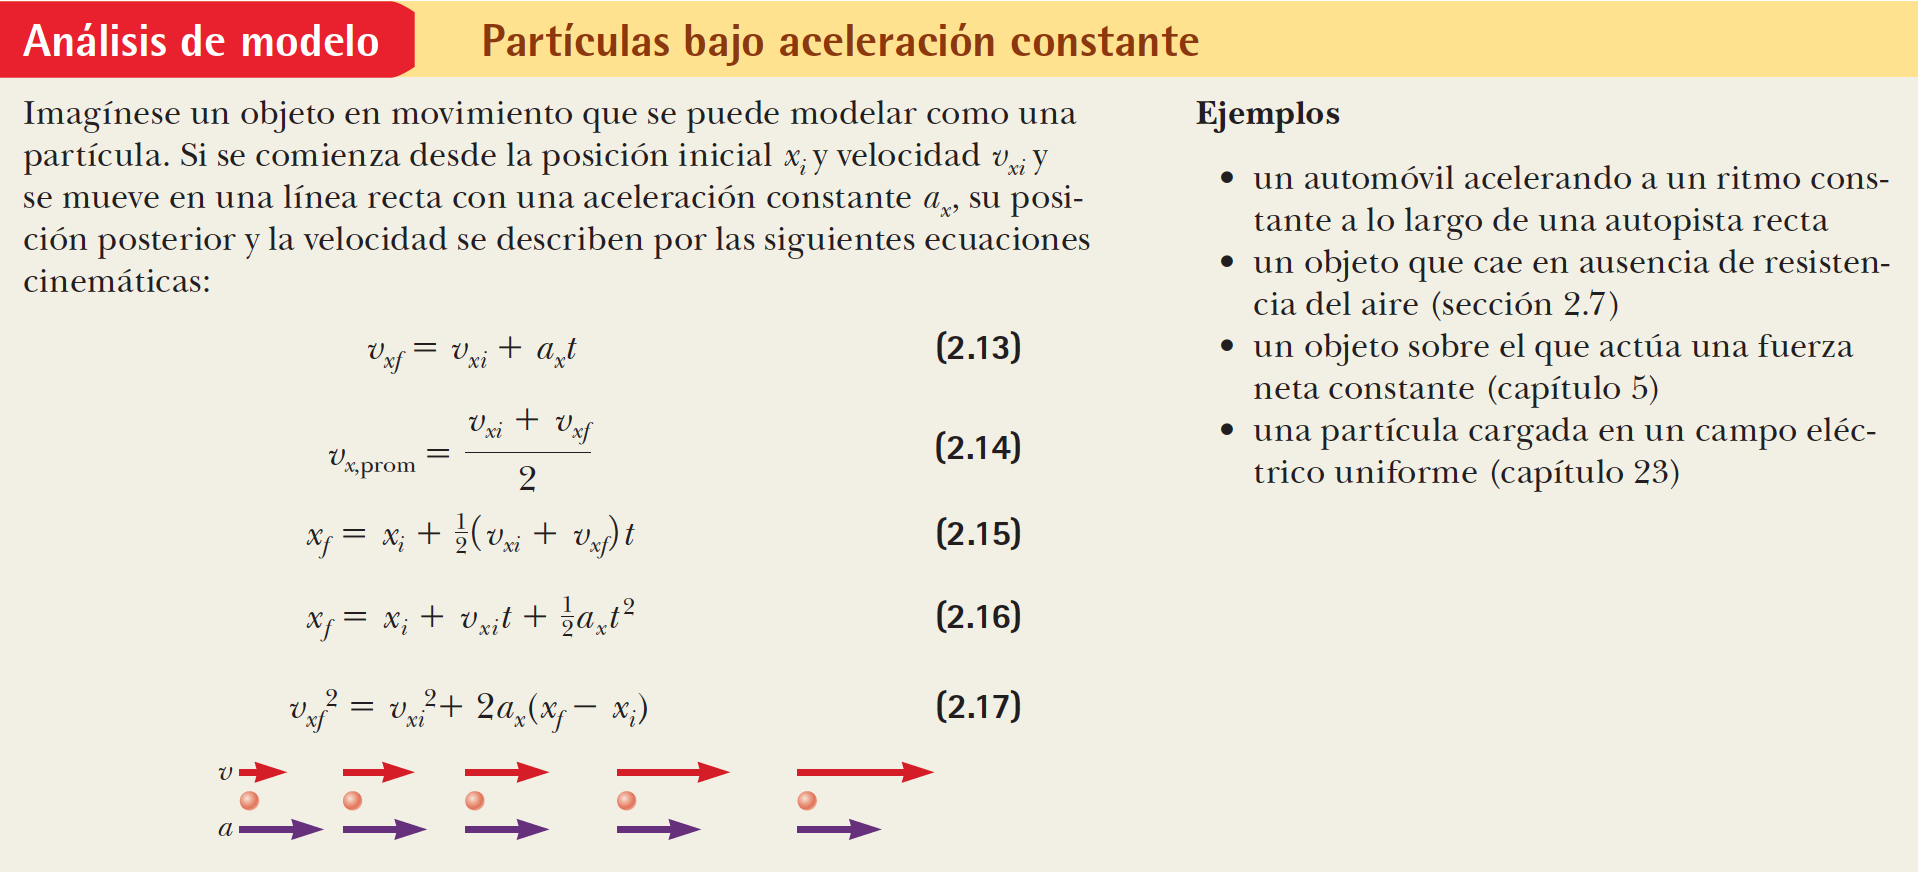
\includegraphics[scale=0.5]{1/graphics_2/figure_0c}
    \end{figure}

  \subsection{Relaciones gráficas entre $x, v_{x}$ y $a_{x}$}
    \begin{figure}[H]
      \centering
      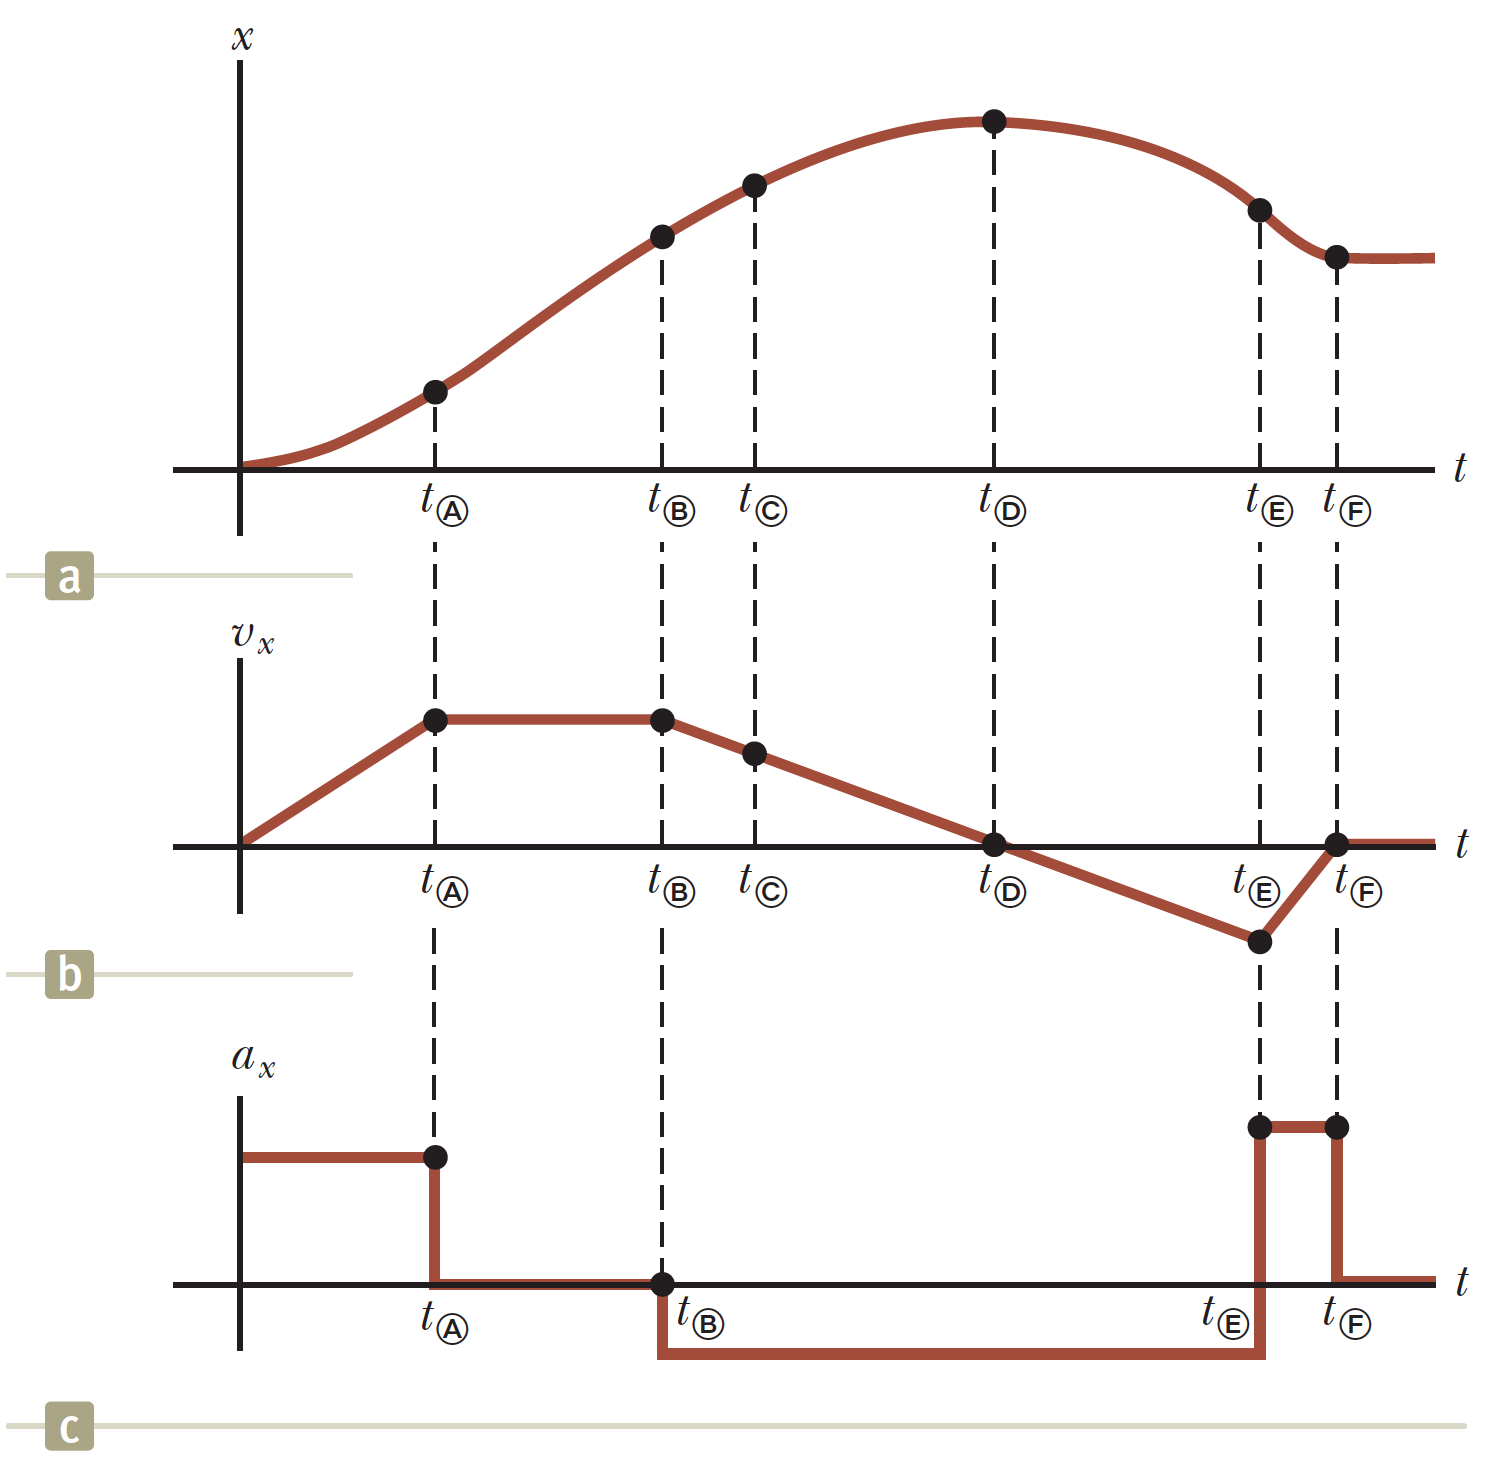
\includegraphics[scale=0.3]{1/graphics_2/figure_1}
      \caption{(a) Gráfica posición-tiempo para un objeto que se mueve a lo largo del eje x. (b) La gráfica
      velocidad-tiempo para el objeto se obtiene al medir la pendiente de la gráfica posición-tiempo en cada instante.
      (c) La gráfica aceleración-tiempo para el objeto se obtiene al medir la pendiente de la gráfica velocidad-tiempo
      en cada instante.}
    \end{figure}

  \subsection{Diagramas de movimiento}
    \PN Con frecuencia los conceptos de \textbf{velocidad} y \textbf{aceleración} se confunden uno con otro, para que
    esto no ocurra, es útil usar una representación pictórica llamada \textit{diagrama de movimiento} para describir la
    velocidad y la aceleración mientras un objeto está en movimiento.

    \begin{figure}[H]
      \centering
      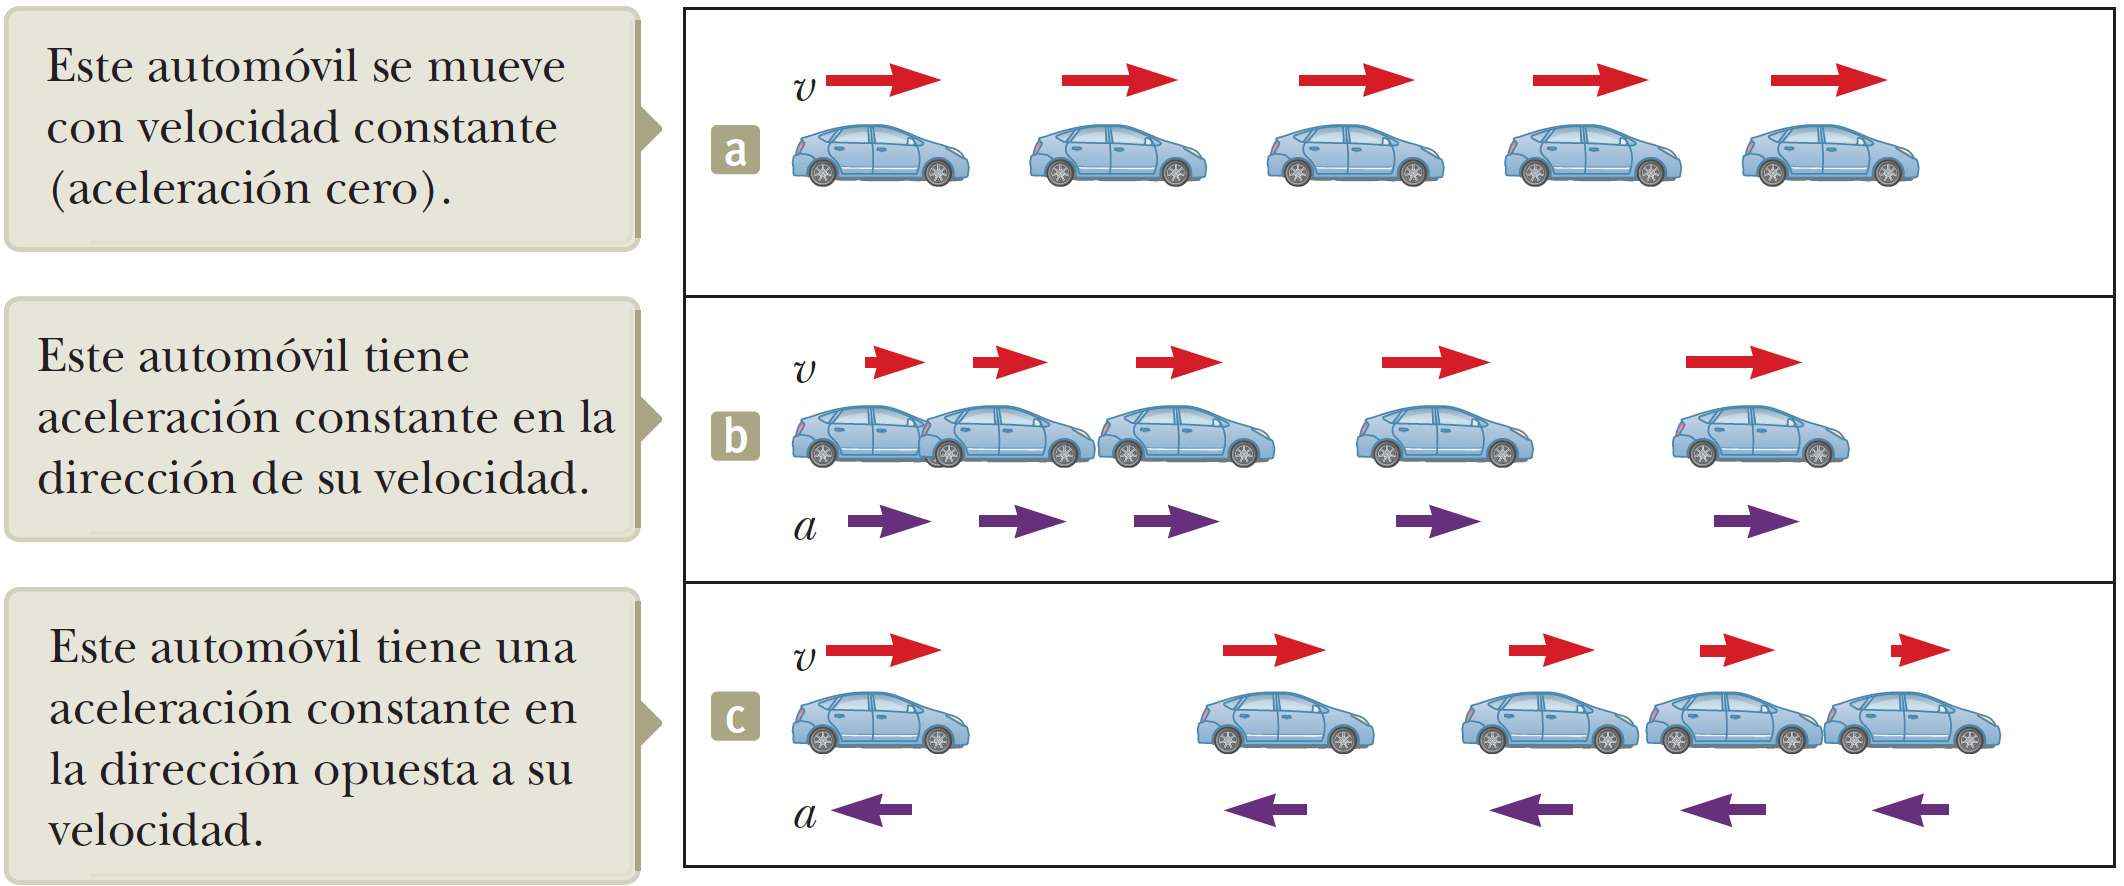
\includegraphics[scale=0.4]{1/graphics_2/figure_2}
      \caption{Diagramas de movimiento de un automóvil que se mueve a lo largo de una carretera recta en una sola
      dirección. La velocidad en cada instante está indicada por una flecha roja, y la aceleración constante se indica
      mediante una flecha de color morado.}
    \end{figure}

  \subsection{Objetos en caída libre}
    \PN En ausencia de resistencia del aire, todos los objetos que se dejan caer cerca de la superficie de la Tierra
    caen hacia ella con la misma aceleración constante bajo la influencia de la gravedad de la Tierra. A dicho
    movimiento se lo conoce como \textit{caída libre}.

    \PN Un objeto en caída libre es cualquier objeto que se mueve libremente sólo bajo la influencia de la gravedad, sin
    importar su movimiento inicial. El movimiento de un objeto en caída libre que se mueve verticalmente es equivalente
    al movimiento de una partícula bajo aceleración constante en una dimensión.
